\documentclass[addpoints]{exam}
\usepackage[utf8x]{inputenc}
\usepackage[ngerman]{babel}
\usepackage{listings}
\usepackage{babel}
\usepackage[top=1.5cm,bottom=0.5cm,headsep=0.5cm,headheight=3cm,%
left=1.5cm,right=1.5cm]{geometry}

\usepackage[T1]{fontenc}
\usepackage{booktabs} % schöne Tabellen
\usepackage{graphicx}
\usepackage{csquotes} % Anführungszeichen
\usepackage{paralist} % kompakte Aufzählungen
\usepackage{amsmath,textcomp,tikz} %diverses
\usepackage{eso-pic} % Bilder im Hintergrund
\usepackage{mdframed} % Boxen
\usepackage{multirow}


\newmdenv[linecolor=black,backgroundcolor=gray!15,
frametitle={Punktverteilung},leftmargin=1cm,
rightmargin=1cm]{infobox}

\lstset{language=Python, tabsize=4, basicstyle=\footnotesize, showstringspaces=false, mathescape=true}
\lstset{literate=%
  {Ö}{{\"O}}1
  {Ä}{{\"A}}1
  {Ü}{{\"U}}1
  {ß}{{\ss}}1
  {ü}{{\"u}}1
  {ä}{{\"a}}1
  {ö}{{\"o}}1
}
\begin{document}
\pointpoints{Punkt}{Punkte}
\bonuspointpoints{Bonuspunkt}{Bonuspunkte}
\renewcommand{\solutiontitle}{\noindent\textbf{Lösung:}%
\enspace}

\chqword{Frage}
\chpgword{Seite}
\chpword{Punkte}
\chbpword{Bonus Punkte}
\chsword{Erreicht}
\chtword{Gesamt}
\hpword{Punkte:} % Punktetabelle
\hsword{Ergebnis:}
\hqword{Aufgabe:}
\htword{Summe:}
\cellwidth{1.5em}
%\begin{center}
%\fbox{\fbox{\parbox{5.5in}{\centering
%Informatik-Klausur}}}
%\end{center}
%
%\vspace{5mm}
%
%\makebox[\textwidth]{Name:\enspace\hrulefill}
\pagestyle{headandfoot}
\runningheadrule

\newcommand\Vtextvisiblespace[1][.3em]{%
  \mbox{\kern.06em\vrule height.3ex}%
  \vbox{\hrule width#1}%
  \hbox{\vrule height.3ex}}

\newcommand{\klaubez}{Aufgaben zu Unicode, UTF8}
\firstpageheader{Informatik }{\klaubez} {\thepage /\numpages}
\runningheader{Informatik }{\klaubez} {\thepage /\numpages}
\newcommand{\pfad}{c:/MyData/07_Kurse/Kursaufgaben}
%-------------------------------------------------------------------
%\printanswers
%-------------------------------------------------------------------

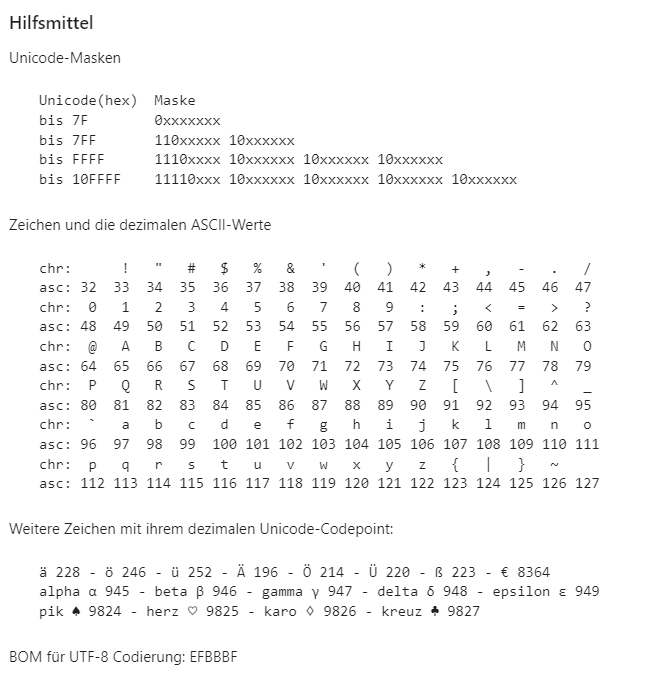
\includegraphics[height=15cm]{\pfad/Unicode/hilfsmittel.png}

\begin{questions}

\input{\pfad/Unicode/utf8_02}
\newpage
\input{\pfad/Unicode/utf8_05}
\input{\pfad/Unicode/welches_zeichen_01}
\input{\pfad/Unicode/welches_zeichen_02}
\newpage
\input{\pfad/Unicode/welches_zeichen_03}






% -------------------------------------------------
\end{questions}
\begin{center}
%\pointtable[h][questions]
\end{center}

\end{document}
